\documentclass[12pt]{pylatex}
\usepackage{examples}
\usepackage{caption}
\usepackage{pgfplots}

\begin{document}

\section*{Plotting Bessel functions}

\vspace{-5pt}

This simple example uses {\tt\small numpy, scipy} and {\tt\small Matplotlib} to produce a plot of the first six Bessel functions. Two plots are shown, one created by {\tt\small Matplotlib} and a second created by LaTeX using the plotting package {\tt\small pgfplots} and the data exported from {\tt\small Matplotlib}.

If you are using macOS, you may need to use the {\tt\small -Ppythonw} option when running {\tt\small pylatex.sh}. This is a known problem with macOS and {\tt\small Matplotlib}, see\ \url{https://matplotlib.org/faq/osx_framework.html}.

\vspace{-10pt}

\begin{minipage}[t]{0.60\textwidth}
\begin{python}
   import numpy as np
   import scipy.special as sp
   import matplotlib.pyplot as plt

   plt.matplotlib.rc('text', usetex = True)
   plt.matplotlib.rc('grid', linestyle = 'dotted')
   plt.matplotlib.rc('figure', figsize = (6.4,4.8)) # (width,height) inches

   x = np.linspace(0, 15, 500)

   for v in range(0, 6):
       plt.plot(x, sp.jv(v, x))

   plt.xlim((0, 15))
   plt.ylim((-0.5, 1.1))
   plt.legend(('${J}_0(x)$', '${J}_1(x)$', '${J}_2(x)$',
               '${J}_3(x)$', '${J}_4(x)$', '${J}_5(x)$'), loc = 0)
   plt.xlabel('$x$')
   plt.ylabel('${J}_n(x)$')
   plt.grid(True)
   plt.tight_layout(0.5)

   plt.savefig('example-04-fig.pdf')

   # save the data for later use by pgfplots
   np.savetxt('example-04.txt',list(zip(x,sp.jv(0,x),sp.jv(1,x),sp.jv(2,x),
                                          sp.jv(3,x),sp.jv(4,x),sp.jv(5,x))),
                               fmt="% .10e")
\end{python}
\end{minipage}
\hskip 0.25cm
\begin{minipage}[t]{0.35\textwidth}
\begin{latex}
   \begin{minipage}{\textwidth}
      \centering
      \IfFileExists{example-04-fig.pdf}%
      {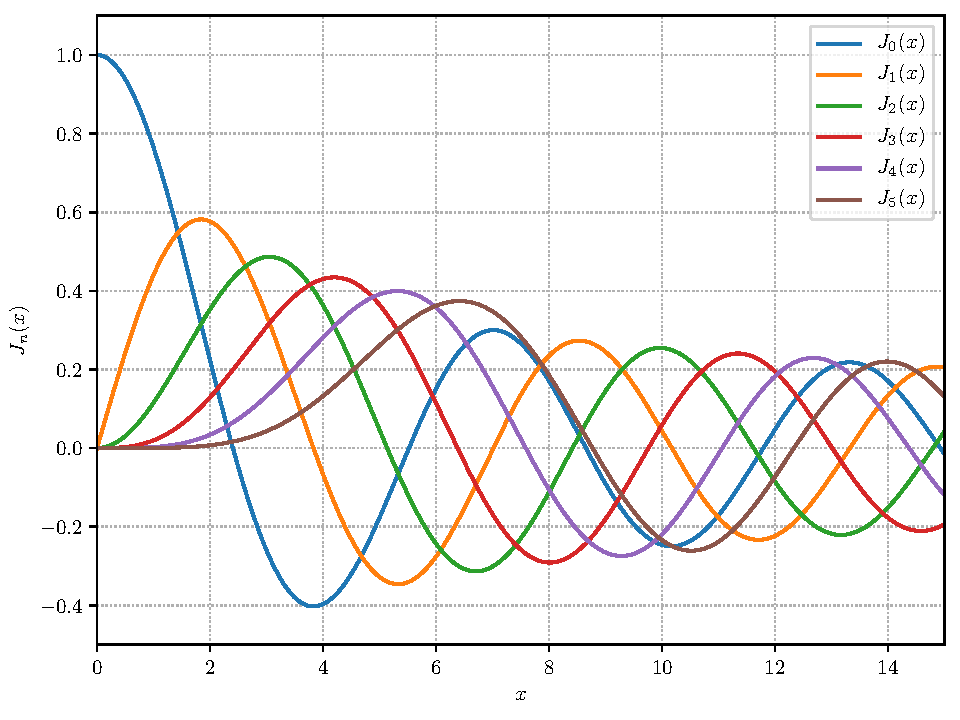
\includegraphics[width=6.4in]
         {example-04-fig.pdf}}{Failed to create pdf plot.}
      \captionof{figure}{The first six Bessel functions.}
   \end{minipage}
\end{latex}
\end{minipage}

\begin{minipage}{\textwidth}
   \centering
   \IfFileExists{example-04-fig.pdf}%
   {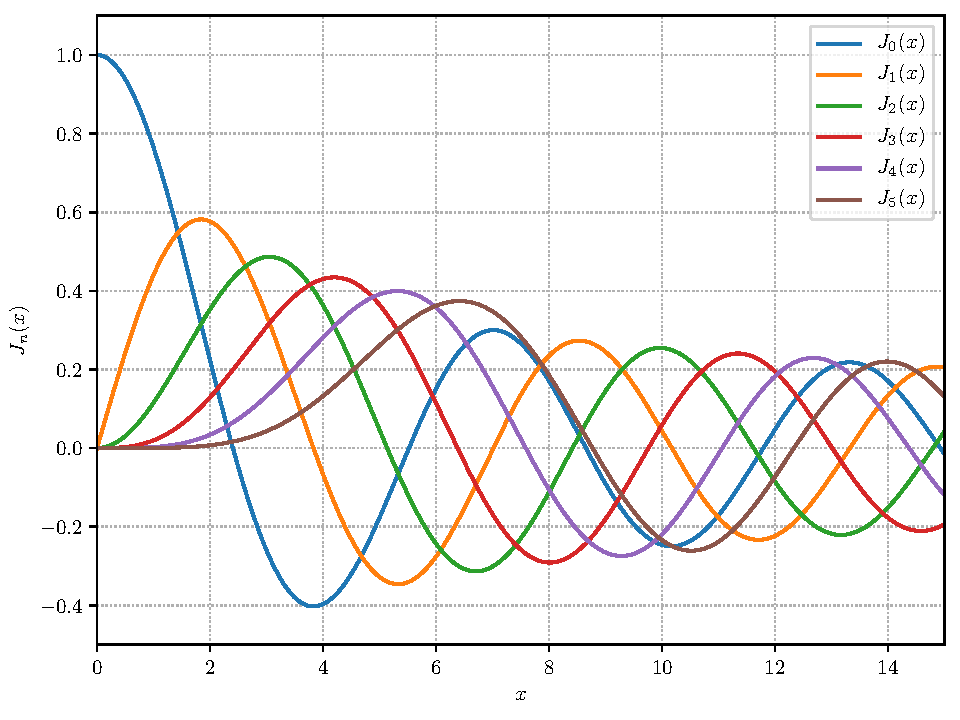
\includegraphics[width=6.4in]
      {example-04-fig.pdf}}{Failed to create pdf plot.}
   \captionof{figure}{The first six Bessel functions.}
\end{minipage}

\clearpage

\pgfplotsset{compat=newest}
\pgfplotsset{width=0.45\textwidth,height=0.34\textwidth}

\subsection*{Using pgfplots}

\begin{minipage}[t]{\textwidth}
   \centering
   \begin{tikzpicture}
      \begin{axis}
         [xmin= 0.0,  xmax=15.0,
          ymin=-0.45, ymax=1.05,
          xlabel=$x$, ylabel=$J_n(x)$,
          grid=major, grid style={dashed,gray!30},
          legend entries = {$J_0$, $J_1$, $J_2$, $J_3$, $J_4$, $J_5$}]
          \addplot[blue]   table [x index=0, y index=1]{example-04.txt};
          \addplot[red]    table [x index=0, y index=2]{example-04.txt};
          \addplot[green]  table [x index=0, y index=3]{example-04.txt};
          \addplot[teal]   table [x index=0, y index=4]{example-04.txt};
          \addplot[orange] table [x index=0, y index=5]{example-04.txt};
          \addplot[purple] table [x index=0, y index=6]{example-04.txt};
      \end{axis}
   \end{tikzpicture}
   \captionof{figure}{The first six Bessel functions.}
\end{minipage}

\vfill

\begin{latex}
   \begin{tikzpicture} % requires \usepackage{pgfplots}
      \begin{axis}
         [xmin= 0.0,  xmax=15.0,
          ymin=-0.45, ymax=1.05,
          xlabel=$x$, ylabel=$J_n(x)$,
          grid=major, grid style={dashed,gray!30},
          legend entries = {$J_0$, $J_1$, $J_2$, $J_3$, $J_4$, $J_5$}]
          \addplot[blue]   table [x index=0, y index=1]{example-04.txt};
          \addplot[red]    table [x index=0, y index=2]{example-04.txt};
          \addplot[green]  table [x index=0, y index=3]{example-04.txt};
          \addplot[teal]   table [x index=0, y index=4]{example-04.txt};
          \addplot[orange] table [x index=0, y index=5]{example-04.txt};
          \addplot[purple] table [x index=0, y index=6]{example-04.txt};
      \end{axis}
   \end{tikzpicture}
   \captionof{figure}{The first six Bessel functions.} % requires \usepackage{caption}
\end{latex}

\end{document}
